\section{機器學習(Machine Learning)}
機器學習為實現人工智慧的一種途徑,利用過往資料歸納出解決問題的方法。例子包括:
機器學習根據有無人為標註資料與否,可分爲監督式學習及非監督式學習兩類;
以下主要介紹監督式學習。
\subsection{機器學習問題架構}
\vspace{12pt}
\noindent\textbf{符號定義}
\vspace{4pt}

我們首先介紹監督式學習所用到的符號:
\begin{itemize}
    \item 輸入(input): $x \in \mathcal{X}$;$\mathcal{X}$代表輸入空間。
    \item 輸出(output): $y: \in \mathcal{Y}$;$\mathcal{Y}$代表輸出空間。
    \item 函數空間(function space): $\mathcal{F} = \{\ f\ |\ f: \mathcal{X} \rightarrow \mathcal{Y} \}$
    \item 資料空間: $\mathcal{D} = \mathcal{X} \times \mathcal{Y}$
    \item 資料集: $D = \{ (x_1, y_1), (x_2, y_2), \ldots, (x_N, y_N)\} \overset{i.i.d.}{\sim} \mathcal{D}$
    \item 假說集合(hypothesis set): $\mathcal{H}, \mathcal{H} \subset \mathcal{F}$
    \item 損失函數(loss function): $\ell: \mathcal{Y} \times \mathcal{Y} \rightarrow \mathbb{R}$
    \item 理想函數(oracle function): $f^{*}: \mathcal{X} \rightarrow \mathcal{Y}\quad s.t.\quad \mathbb{E}_{x, y \sim \mathcal{D}}\left[\ell(f^{*}(x), y)\right] = 0$
    \item 學習演算法(learning algorithm):  $a: \left( \mathcal{H}, D \right) \mapsto h,\quad h \in \mathcal{H}$
\end{itemize}
\vspace{12pt}
\noindent\textbf{輸入與輸出}
\vspace{4pt}

輸入與輸出的例子包括:
\begin{itemize}
    \item 銀行根據過往核發信用卡的申請人的背景及是否批准核發的資料。$x$:申請人背景;$y$:核發與否。
    \item 新聞分類。$x$:新聞內容;$y$:新聞類別,如政治、體育。
    \item 影像分類。$x$:影像;$y$:影像類別,如貓、狗。
\end{itemize}
\vspace{12pt}
\noindent\textbf{損失函數}
\vspace{4pt}

定義好輸入與輸出之後,我們需要給定衡量模型輸出與正確答案的偏差的函數,稱為損失函數$\ell({\cdot},{\cdot})$;常見的任務及其損失函數羅列如下:
\begin{itemize}
    \item 二元分類(binary classification):$\mathcal{Y} = \{0, 1\}$
    \begin{itemize}
        \item 0-1 損失函數(0-1 loss function):\\
        $
            \ell(\hat{y}, y) = \begin{dcases*}
                                1 & if $\hat{y} \neq y$ \\
                                0 & if $\hat{y} = y$
                                \end{dcases*}
        $
        \item 交叉熵函數(cross-entropy function):\\
        $
            \ell(\hat{y}, y) = y \cdot \log p(\hat{y}) + (1 - y) \cdot \log (1 - p(\hat{y})),\\
            \hat{y} = \begin{dcases*}
                1 & if $p(\hat{y}) > 0.5,$ \\
                0 & otherwise
                \end{dcases*}
        $
    \end{itemize}
    \item 多元分類(multiclass classification):$\mathcal{Y} = \{0, 1, \ldots, N\}$
    \begin{itemize}
        \item 交叉熵函數:\\
        $
            \ell(\hat{y}, y) = \sum_{i=1}^{N} y_{i} \log (\hat{y}_{i}),\\
            y_i = \begin{dcases*}
                    1 & if $y = i,$ \\
                    0 & if $y \neq i$
                  \end{dcases*}
        $
    \end{itemize}
\end{itemize}
\vspace{12pt}
\noindent\textbf{學習演算法}
\vspace{4pt}

給定輸入資料與相對應的答案,監督式學習的學習演算法$a$的目標是在假說集合$\mathcal{H}$內尋找損失函數在資料分佈$\mathcal{D}$上的期望值最小:
\begin{equation}
h^{*} = \argmin_{h \in \mathcal{H}}\ \mathbb{E}_{x, y \sim \mathcal{D} } \left[ \ell (h(x), y) \right]
\end{equation}
但資料的變化千千萬萬,我們得不到世界上所有的資料,因此我們並不知道真實的資料分佈$\mathcal{D}$,
只能用蒐集到的資料集$D = \{\left(x_i, y_i \right)\}_{i=1}^{N}$去近似它:
\begin{equation}
    h^{*} = \argmin_{h \in \mathcal{H}}\ \frac{1}{N} \sum\limits_{i=1}^{N} \ell (h(x_i), y_i)
\end{equation}
\subsection{機器學習模型}
機器學習中所謂的模型通常包含了假說集合、學習演算法、與其配合的損失函數。以下列舉常見的模型及其組成:
\begin{itemize}
    \item 支撐向量機:
    \begin{itemize}
        \item 假說集合:徑向基函數(radial basis function)、多項式(polynomial)等
        \item 學習演算法:二次規劃(quadratic programming)
        \item 損失函數:鉸接損失函數(hinge loss)
    \end{itemize}
    \item 類神經網路:
    \begin{itemize}
        \item 假說集合:類神經網路
        \item 學習演算法:梯度下降(gradient descent)
        \item 損失函數:交叉熵函數(cross-entropy loss)用於多元分類、均方差函數(MSE loss)用於迴歸(regression)等
    \end{itemize}
\end{itemize}

\section{深度類神經網路(Deep Neural Networks)}
深度類神經網路為一種仿造生物神經網路的計算模型,具有強大的建模能力,及可以近似任意連續函數的理論保證\cite{hornik1991approximation},
過去數十年由於電腦計算能力的不足而造成研究進展緩慢;不過自2000年代中期以後,隨著電腦算力逐漸增強而逐漸在圖像、語音領域取得優異的成績。
其架構仿造動物神經元的設計,每個神經元會接收來自其他數個神經元 $x_1, x_2, \ldots, x_n$ 的訊號,將這些訊號依自身的權重 $w_1, w_2, \ldots, w_n$ 加權後加上偏差 $b$ ,
最後通過激活函數 $\sigma: \mathbb{R} \rightarrow \mathbb{R}$ 決定該神經元的輸出 $y = \sigma \left( \sum\limits_{i=1}^{n} w_i x_i + b \right)$ ,傳遞給下個神經元。

\subsection{前饋式類神經網路(FeedForward Neural Network)}
前饋式類神經網路(FeedForward Neural Network)為早發明、也是最簡單的一種類神經網路,可分爲單層與多層前饋式類神經網路。

單層的類神經網路由權重(weight)$\mathbf{W}$、偏差(bias)$\mathbf{b}$ 與激活函數(activation function) $f$ 所組成。
其運作方式接受輸入神經元組(向量) $\mathbf{x}_{in} \in \mathbb{R}^{n}$ ,將其乘以權重 $\mathbf{W} \in \mathbb{R}^{m \times n}$ ,
加上偏差 $\mathbf{b} \in \mathbb{R}^{m}$ ,最後通過激活函數 $f$ 得到輸出神經元組(向量) $\mathbf{x}_{out} \in \mathbb{R}^{m}$ :
\begin{equation}
    \mathbf{x}_{out} = f(\mathbf{W} \mathbf{x}_{in} + \mathbf{b})
\end{equation}

多層類神經網路則將多個單層類神經網路連接起來,將一單層類神經網路的輸出神經元組作為下層類神經網路的輸入神經元組:
\begin{equation}
    \mathbf{x}_{\ell} = f(\mathbf{W} \mathbf{x}_{\ell-1} + \mathbf{b})
\end{equation}
因此給定一L層類神經網路、輸入神經元組$\mathbf{x}_{0}$、及輸出神經元組$\mathbf{y}$,該類神經網路計算方式如下:
\begin{equation}
    \begin{split}
    \mathbf{x}_{1} &= f_{1}(\mathbf{W}_{1} \mathbf{x}_{0} + \mathbf{b}_{1}) \\
    \mathbf{x}_{2} &= f_{2}(\mathbf{W}_{2} \mathbf{x}_{1} + \mathbf{b}_{2}) \\
    \mathbf{x}_{3} &= f_{3}(\mathbf{W}_{3} \mathbf{x}_{2} + \mathbf{b}_{3}) \\
    \vdots \\
    \mathbf{x}_{L} &= f_{L}(\mathbf{W}_{L} \mathbf{x}_{L-1} + \mathbf{b}_{L}) \\
    \end{split}
\end{equation}
在所有的類神經網路裡,激活函數必須是非線性的函數,否則根據線性函數的性質,線性激活函數所組成的多層類神經網路只等價於一簡單的仿射變換。
%非線性函數由於歷史上強調其與動物神經網路的相似而又稱為激活函數(activation function)。
\subsection{類神經網路訓練(Deep Neural Network Training)}
訓練類神經網路通常使用梯度下降法(gradient descent)來進行模型的優化(optimization)。
給定模型參數 $\theta$、模型函數 $h_{\theta}$、損失函數 $\ell$、輸入 $\mathbf{x}$、正確輸出 $\mathbf{y}$、更新過後的參數$\theta'$,
梯度下降法更新參數的公式如下:
\begin{equation}
    \theta' = \theta - \alpha \frac{\partial \ell(h_{\theta}(\mathbf{x}), \mathbf{y})}{\partial \theta}
\end{equation}
其中$\alpha$為梯度下降的步數大小,稱為學習率(Learning rate),太大則可能錯過局部最佳點,太慢則缺乏效率,需要細心調整。

如果進行梯度下降法時使用整個資料集的資料,則稱為批次梯度下降(batch gradient descent):
\begin{equation}
    \theta' = \theta - \alpha \frac{ \partial \sum\limits_{i=1}^{N} \ell\left(h_{\theta}\left(\mathbf{x}_{i}\right), \mathbf{y}_{i}\right)}{\partial \theta}
\end{equation}

當損失平面(loss surface)接近convex、或有一全域最優點的時候,批次梯度下降可以迅速找到該點,獲得好的結果;
但當損失平面高度非convex、並有很多局部最優點的時候,梯度下降法(gradient descent)缺乏逃出不夠好的局部最優點的隨機性,
因而需要隨機梯度下降法(stochastic gradient descent)來提供隨機性:
\begin{equation}
    \theta' = \theta - \alpha \frac{ \partial \ell\left(h_{\theta}\left(\mathbf{x}_{i}\right), \mathbf{y}_{i}\right)}{\partial \theta}
\end{equation}

隨機梯度下降法每次更新只用一筆資料,計算出的梯度較雜亂(noisy),優點是使參數有機會逃出局部最優點,缺點則是梯度太過雜亂,
且一次只使用一筆資料,無法利用圖形處理器(Graphics Processing Unit, GPU)平行處理所帶來的速度優勢縮短訓練時間;
小批次隨機梯度下降法(mini-batch stochastic gradient descent)則將一次更新所使用的資料數設於上述兩者之間:
\begin{equation}
    \theta' = \theta - \alpha \frac{ \partial \sum\limits_{i=1}^{N'} \ell\left(h_{\theta}\left(\mathbf{x}_{i}\right), \mathbf{y}_{i}\right)}{\partial \theta}
\end{equation}
其中$1 \ll N' \ll N$。小批次隨機梯度下降法不若批次梯度下降法缺乏隨機性,也沒有隨機梯度下降法太隨機且過慢的缺點,爲現行主流機器學習界採用的方法。


\subsection{遞歸式類神經網路(Recurrent Neural Network)}
遞歸式類神經網路為一種接受序列為輸入的類神經網路,特別適合處理自然語言、語音、音樂等序列資料。其特色在於資料並不是一次全部輸入網路,
而是依照序列自身的排序一一輸入網路;而網路除了接受當前時間點的輸入$\mathbf{x}_t$之外,還另外接受前一個時間點的隱含狀態$\mathbf{h}_{t-1}$,
處理後得到這個時間點的隱含狀態 $\mathbf{h}_{t}$ 與模型輸出 $\mathbf{y}_{t}$ 。

\vspace{12pt}
\noindent\textbf{艾氏遞歸式類神經網路(Elman RNN)}
\vspace{4pt}

首先我們介紹最基本的由艾氏(Jeffrey L. Elman)於1990年提出的艾氏遞歸式類神經網路\cite{elman1990finding}:
給定在t時間點的隱含狀態$\mathbf{h}_{t} \in \mathbb{R}^{m}$、序列資料$\{\mathbf{x}_i\}_{i=1}^{T},\ \mathbf{x}_t \in \mathbb{R}^{n}$,
輸出向量$y_{t} \in \mathbb{R}^{o}$,
艾氏遞歸式類神經網路的運作方式如下:
\begin{equation}
    \begin{split}
    \mathbf{h}_{t} &= \sigma_{h} \left( \mathbf{W}_{h} \mathbf{x}_{t} + \mathbf{U}_{h} \mathbf{h}_{t-1} + \mathbf{b}_h \right) \\
    \mathbf{y}_{t} &= \sigma_{h} \left( \mathbf{W}_{y} \mathbf{h}_{t-1} + \mathbf{b}_y \right)
    \end{split}
\end{equation}
其中$\mathbf{W}_{h} \in \mathbb{R}^{m \times n}$、
$\mathbf{U}_{h} \in \mathbb{R}^{m \times m}$、
$\mathbf{W}_{h} \in \mathbb{R}^{m \times n}$、
$\mathbf{W}_{y} \in \mathbb{R}^{o \times n}$。

\vspace{12pt}
\noindent\textbf{長短期記憶遞歸式類神經網路(LSTM RNN)}
\vspace{4pt}

長短期記憶遞歸式類神經網路(Long-Short Term Memory RNN, LSTM RNN)由施氏(Jürgen Schmidhuber)\cite{hochreiter1997long}於1997年提出,
將閘門(gate)的概念引入遞歸式類神經網路來控制資訊的流動,取得巨大的成功。總共有三個閘門用來控制LSTM中資訊的流動:
輸入閘(input gate)、輸出閘(output gate)、遺忘閘(forget gate)。
\begin{subequations}
    \begin{align}
    \mathbf{i}_t &= \sigma_{g} \left( \mathbf{W}_i \mathbf{x}_t + \mathbf{U}_i \mathbf{h}_{t-1} + \mathbf{b}_i \right) \\
    \mathbf{o}_t &= \sigma_{g} \left( \mathbf{W}_o \mathbf{x}_t + \mathbf{U}_o \mathbf{h}_{t-1} + \mathbf{b}_o \right) \\
    \mathbf{f}_t &= \sigma_{g} \left( \mathbf{W}_f \mathbf{x}_t + \mathbf{U}_f \mathbf{h}_{t-1} + \mathbf{b}_f \right) \\
    \mathbf{\tilde{c}}_{t} &= \sigma_{h} \left( \mathbf{W}_c \mathbf{x}_t + \mathbf{U}_c \mathbf{h}_{t-1} + \mathbf{b}_c \right) \\
    \mathbf{c}_{t} &= \mathbf{f}_t \circ \mathbf{c}_{t-1} + \mathbf{i}_t \circ \mathbf{\tilde{c}}_t \\
    \mathbf{h}_t &= \mathbf{o}_t \circ \sigma_{h} (\mathbf{c}_t)
    \end{align}
\end{subequations}
其中$\mathbf{x}_t$為輸入向量、
$\mathbf{f}_t$為遺忘閘向量、
$\mathbf{i}_t$為輸入閘向量、
$\mathbf{o}_t$為輸出閘向量、
$\mathbf{h}_t$為隱含狀態向量、
$\mathbf{c}_t$為單元狀態(cell state)向量、
$\sigma_{g}$為sigmoid函數、
$\sigma_{h}$為tanh函數。
LSTM用輸入閘來控制要讓多少輸入向量的資訊流入單元狀態向量;
遺忘閘向量用來決定要留住/遺忘多少上個時間點的單元狀態向量;
輸出閘向量則負責控制單元狀態的資訊有多少流入隱含狀態向量。
\subsection{轉換器類神經網路(Transformer Neural Network)}
轉換器類神經網路為梵氏(Ashish Waswani)等人\cite{NIPS2017_7181}於2017年提出,捨棄了常被詬病時間點之間無法平行處理而顯得過慢的遞歸式結構,
轉而使用可以平行計算的自專注機制(self-attention mechanism)作爲模型的主架構,在2017年之後蔚爲流行,頗有取代遞歸式類神經網路之勢。

\vspace{12pt}
\noindent\textbf{自專注機制(Self-Attention Mechanism)}
\vspace{4pt}

我們首先介紹自專注機制:以輸入層(input layer)為例,
嵌入層(embedding layer)將$\MWord_{i}$編碼成
詢向量(query vector)$q_i \in \mathbb{R}^{d_k}$、
鑰向量$k_i \in \mathbb{R}^{d_k}$
與值向量$v_i\in \mathbb{R}^{d_v}$;
則自專注模組會輸出該字 $\MWord_{i}$ 對句子中其他字的專注權重。定義$\alpha_{ij}$為$\MWord_{i}$對$\MWord_{j}$的專注權重,則
\begin{equation}
    \alpha_{ij} = \mathrm{softmax} \left( \frac{q_i k_j^{\top}}{\sqrt{d_k}} \right)
                = \frac{\mathrm{exp}(\frac{q_i k_j^{\top}}{\sqrt{d_k}})}{\sum_{j'=1}^{N} \mathrm{exp}(\frac{q_i k_j'^{\top}}{\sqrt{d_k}})}
\end{equation}
特別的是,詢向量與鑰向量之間的內積$q_i k_j^{\top}$會先除以$\sqrt{d_k}$,再送入軟性最大化層(softmax layer);
這是為了確保當詢與鑰向量的維度$d_k$變大,內積的大小不會跟著變大,使得通過軟性最大化層後產生梯度消失(gradient vanishing)的現象而妨害訓練;
瓦氏將此專注機制稱為縮放式點積專注法(Scaled Dot-Product Attention)。
自專注對 $\MWord_{i}$ 的輸出$y$則為此權重對所有字的值向量 $v$ 的加權之和:
\begin{equation}
    y = \sum\limits_{j=1}^{N} \alpha_{ij} v_j
\end{equation}
將句子中所有字的詢向量、鑰向量與值向量組合成矩陣(如
$
V =
\begin{bmatrix}
    v_1   & v_2   & \dots & v_N
\end{bmatrix}
$),我們可以寫出自專注機制的矩陣形式:
\begin{equation}
    \mathrm{SelfAtt}(Q, K, V) = \mathrm{softmax} \left(\frac{Q K^{\top}}{\sqrt{d_{k}}} \right) V
\end{equation}
事實上,自專注機制是一種圖神經網路的特例:
圖神經網路的每個節點透過對與其有連結的其他節點進行互動來更新自己的表示(representation);
自專注機制則可以視為一個以字為節點的全連接圖(fully-connected graph)的圖神經網路。
%因此在圖神經網路的框架下,自專注機制的運作方式直覺上可以解釋成:自身的詢向量與所有字的鑰向量

\vspace{12pt}
\noindent\textbf{多頭自專注(Multi-Head Self Attention)}
\vspace{4pt}

梵氏在同篇論文中發現使用多組不同的專注模組,對效能有正面的提升;因此他提出多頭自專注,
將維度為$d_{\mathrm{model}}$的詢向量、鑰向量與值向量線性投影到多個維度為$d_k$、$d_k$、$d_v$的子空間(subspace),
在子空間中分別進行自專注機制運算後,再將他們重組起來並投影回維度為$d_{\mathrm{model}}$的空間:
\begin{equation}
    \begin{split}
    \mathrm{MultiHead}(Q, K, V) &= \mathrm{Concat} (\mathrm{head}_{1}, \ldots, \mathrm{head}_{h}) W^{O} \\
        \text{其中}\mathrm{head}_{i} &= \mathrm{Attention} (QW_{i}^{Q}, KW_{i}^{K}, VW_{i}^{V})
    \end{split}
\end{equation}
投影矩陣的維度分別為
$W_{i}^{Q} \in \mathbb{R}^{d_{\mathrm{model}} \times d_{k}}$,
$W_{i}^{K} \in \mathbb{R}^{d_{\mathrm{model}} \times d_{k}}$,
$W_{i}^{V} \in \mathbb{R}^{d_{\mathrm{model}} \times d_{v}}$,
$W^{O} \in \mathbb{R}^{hd_{v} \times d_{\mathrm{model}}}$。
之後的研究發現多頭自專注有利於模型對不同的語言現象,如詞的位置、不同語法功能、少見詞等分別進行專注機制運算\cite{voita-etal-2019-analyzing}。

\vspace{12pt}
\noindent\textbf{位置編碼(Positional Encoding)}
\vspace{4pt}

由於自專注機制不若遞歸式類神經網路,透過輸入網路的先後順序暗中給了網路字與字的相對位置資訊,自專注機制若沒有特別的模組為每個字的位置建模,
有序的字組成的句子與無序的詞袋(bag-of-words)並無二致。因此梵氏引入位置編碼,直接將位置資訊以向量的形式表示:

\begin{equation}
    \begin{split}
    {PE}_{\mathrm{pos},\mathrm{2i}} = \sin (\mathrm{pos} / 10000^{2i / d_{\mathrm{model}}}) \\
    {PE}_{\mathrm{pos},\mathrm{2i}+1} = \cos (\mathrm{pos} / 10000^{2i / d_{\mathrm{model}}})
    \end{split}
\end{equation}
其中$\mathrm{pos}$代表位置,而$i$代表維度。使用正弦與餘弦函數的優點,梵氏的解釋是模型可以透過這些函數的週期性學習字與字的相對位置。

\section{分佈式表示(distributed representation)}
如何將語義以電腦可理解的方式表示,可以說是自然語言處理的核心問題。
以下介紹最爲流行的一派方法,也就是以分佈式語義學(distributional semantics)為基礎的分佈式表示。



\subsection{詞向量(Word Vectors)}

最簡單的方法為尋找一個足夠有代表性的語料庫,經過分詞後,統計詞與詞之間共同出現的次數,構建出詞之間的共現矩陣。
底下用只有四句話的語料展示如何構建共現矩陣(co-occurrence matrix):
\begin{itemize}
\item 李宏毅 幾 班 ?
\item 李宏毅 五 年 二十 班 。
\item 李仲翊 幾 班 ?
\item 李仲翊 三 年 五 班 。
\end{itemize}
以上四句話的共現矩陣為:
\begin{table}[ht]
    \center
    \begin{tabular}{|c|c|c|c|c|c|c|c|c|} \hline
    %\begin{tabularx}{\textwidth}{|*{9}{X|}} \hline
           & 李宏毅 & 李仲翊 & 幾 & 班 & 三 & 五 & 年 & 二十  \\ \hline
     李宏毅 & 0 & 0 & 1 & 2 & 0 & 1 & 1 & 1 \\ \hline
     李仲翊 & 0 & 0 & 1 & 2 & 1 & 1 & 1 & 0 \\ \hline
        幾 & 1 & 1 & 0 & 2 & 0 & 0 & 0 & 0 \\ \hline
        班 & 2 & 2 & 2 & 0 & 1 & 2 & 2 & 1 \\ \hline
        三 & 0 & 1 & 0 & 1 & 0 & 1 & 1 & 0 \\ \hline
        五 & 1 & 1 & 0 & 2 & 1 & 0 & 2 & 1 \\ \hline
        年 & 1 & 1 & 0 & 2 & 1 & 2 & 0 & 1 \\ \hline
      二十 & 1 & 0 & 0 & 1 & 0 & 1 & 1 & 0 \\ \hline
    \end{tabular}
    %\end{tabularx}
    \caption{共現矩陣的示例。}
    \label{tab:cooccur}
\end{table}

表\ref{tab:cooccur}中,每個字的分佈表示即爲該欄/列向量(在對稱的共現矩陣中欄向量與列向量相同)。

但此共現矩陣的大小為語料庫中詞種數的平方:若詞種數為$|V|$,則共現矩陣大小為${|V|}^{2}$,
這樣的矩陣過於龐大(矩陣內每格均爲整數,若一整數有 4 bytes,詞種數為100,000,則此矩陣共有$4 \times 100,000 \times 100,000 = 4$ GB),
其隱含的資訊量應能用更少的維度表示;
因此後人提出許多降維(Dimension Reduction) 配合矩陣平滑化(Smoothing)(或可達成類似目的)的方法得出低維度的詞向量,
以下舉最成功的文字向量(Word2Vec)為例:
\iffalse
這裏舉兩個例子介紹,分別為文字向量(Word2Vec)及全局向量詞表示(GloVe)。
\fi

\vspace{12pt}
\noindent\textbf{Word2Vec}
\vspace{4pt}

文字向量(word2vec)為米氏(mikolov)於2013年提出及開發,
以批次訓練分解共現矩陣$M$(co-occurrence matrix)為詞矩陣$W$及語境(context)矩陣$C$,
其優點是不需要事先統計並儲存龐大的共現矩陣(若有十萬詞,則$\text{矩陣大小} = 100,000^{2} $ ),
每次分批讀入小部分語料後更新 $W$ 及 $C$ 即可。損失函數方面,捨棄需要更新所有詞參數的軟性最大化(softmax),
而使用噪聲對比估計(Noise Contrastive Estimation)損失函數,有效降低計算負擔。
其運作方式如下:

給定一詞$w$及其語境$c$,文字向量的目標旨在最大化該詞的詞向量 $\vec{w}$ 及該語境的語境向量 $\vec{c}$ 的內積;
具體的機率模型則使用S函數(sigmoid function)來表示詞-語境對$(w, c)$(word-context pair)出現在語料庫$D$的機率:
\begin{equation}
P(D=1|w,c) = \sigma (\vec{w} \cdot \vec{c}) = \frac{1}{1 + e^{-\vec{w} \cdot \vec{c}}}
\end{equation}

若只有最大化出現在語料庫中詞-語境對$(w, c)$,到最後所有 $\vec{w}$ 與 $\vec{c}$ 都會朝向同個方向,這不是我們所希望得到的詞向量,
因此還需要做負取樣(negative sampling),也就是隨機取樣不會出現在語料庫裡的負樣本$(\vec{w}, \vec{c_{N}})$並降低其出現的機率
(實際操作上並不會檢查隨機從詞彙裡取樣語境$\vec{c_{N}}$得到的詞-語境對$(w, \vec{c_{N}})$是否出現在語料庫$D$,而直接假定出現的機率不大)。
因此詞向量的損失函數如下:

\begin{equation}
    \ell = - \sum\limits_{w \in V_{W}} \sum\limits_{c \in V_{C}} \#(w, c) \left( \log \sigma (\vec{w}, \vec{c}) + k \cdot \mathbb{E}_{c_{N} \sim P_{D}} [\log \sigma \left( - \vec{w}, \vec{c_{N}} \right)] \right)
\end{equation}

其中$k$為每個正樣本搭配的負樣本的個數,
$\#(w, c)$為詞-語境對$(w, c)$出現在語料庫$D$中的次數,
$\vec{c_{N}}$為取樣自一元分佈(unigram distributation) $P_{D} (c) = \frac{\#(c)}{|D|}$ 的語境詞。

文字向量取得了巨大的成功,從2014年到2018年都是各種自然語言處理任務的標準配備,直到上下文化表示的出現(見章節\ref{subsec:cxtrep})。

\iffalse
\vspace{12pt}
\noindent\textbf{全局向量詞表示(GloVe)}
\vspace{4pt}
GloVe使用矩陣分解(matrix factorization)將碩大無朋的共現矩陣$M$分解為兩個子矩陣$W$與$C$,根據其設計的損失函數:
\fi

\subsection{語境化表示(Contextualized Representations)}
詞向量在各種自然語言處理任務中雖然取得了巨大的成功,其一詞一向量的本質並不適合處理多義詞、代名詞指涉、或甚至同一詞其語義在不同語境下的微妙差異。
為了解決這樣的問題,研究者開始思考一詞多個向量的可能性,如詞義向量(word sense embeddings),
給予不同詞義不同的向量(如bank有河岸或銀行兩種意思)\cite{reisinger-mooney-2010-multi,neelakantan-etal-2014-efficient}。
而將一詞多向量的想法推行到極致,就是語境化表示的想法:對同一詞,只要出現在不同語境,就給予不同的向量。

\vspace{12pt}
\noindent\textbf{ELMo}
\vspace{4pt}

馬氏\cite{peters-etal-2018-deep}於2018年提出的ELMo (Embeddings from Language Models)為第一個使用語境化表示得到巨大成功的模型,
展示了普通的兩層雙向LSTM(詞嵌入使用字符CNN)用語言模型的目標函數訓練在大量語料上,其隱藏層即蘊含了豐富的語境化表示,
使得ELMo在六種自然語言處理任務相對於基準模型有6\%到20\%的進步率。


\vspace{12pt}
\noindent\textbf{BERT}
\vspace{4pt}

在這之後許多試圖改進ELMo的語境化表示模型如雨後春筍般相繼出現,
如GPT\cite{radford2018improving}、ULMFit\cite{howard2018universal}等,其中最成功且流行的當屬
2019年戴氏\cite{devlin-etal-2019-bert}基於轉換器的架構設計的
轉換器模型的雙向編碼器表示(Birectional Encoder Representations from Transformers, 下稱BERT)。
過去的語境化表示如ELMo、GPT\cite{radford2018improving}等語境化表示通常為單向(unidirectional)語言模型,
而傳統的雙向LSTM語言模型也只是左到右與右到左語言模型的淺層級聯(concatenation),其本質仍是兩個獨立訓練的單向語言模型。
BERT改進了傳統的雙向LSTM語言模型,利用轉換器模型的架構優勢設計了遮蔽式語言模型(masked language model),
相當於給模型進行克漏字測驗的訓練,或也可以看成去噪自編碼器(denoising autoencoder)的一個例子,使模型可以同時利用雙邊的語境進行預測,
使其隱藏層蘊含的訊息更為豐富,而這是兩個各只利用單邊語境的傳統雙向語言模型不能做到的。

\label{subsec:cxtrep}
\section{依存句法剖析(Dependency Parsing)}
\subsection{句法簡介}
\begin{figure}[hb]
  \centering
  \begin{subfigure}[b]{.22\textwidth}
    \centering
    \begin{tikzpicture}
      \Vertices{figs/chapter2/mtt/mtt-vertices-sem.csv}
      \Edges{figs/chapter2/mtt/mtt-edges-sem.csv}
    \end{tikzpicture}
    \caption{SemR}
  \end{subfigure}
  \begin{subfigure}[b]{.22\textwidth}
    \centering
    \begin{tikzpicture}
      \Vertices{figs/chapter2/mtt/mtt-vertices-syn.csv}
      \Edges{figs/chapter2/mtt/mtt-edges-syn.csv}
    \end{tikzpicture}
    \caption{SyntR}
  \end{subfigure}
  \begin{subfigure}[b]{.22\textwidth}
    \centering
    \begin{tikzpicture}
      \Vertices{figs/chapter2/mtt/mtt-vertices-morph.csv}
      \Edges{figs/chapter2/mtt/mtt-edges-morph.csv}
    \end{tikzpicture}
    \caption{MorphR}
  \end{subfigure}
  \begin{subfigure}[b]{.22\textwidth}
    \centering
    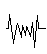
\includegraphics{figs/chapter2/mtt/wave.png}
    \caption{PhonR}
  \end{subfigure}
  \caption{語義-文字理論。}
  \label{fig:mtt}
\end{figure}
句法(syntax)可定義為支配句子結構,決定詞、子句如何組成其上級結構的一系列規則。
根據梅氏(Igor Mel’čuk)的文字-語意理論(Meaning-text theory, 見圖\ref{fig:mtt}),
一段語句的生成可以被描述為從語意表徵(semantic representation, SemR)到語音表徵(phonetic representation, PhonR)之間一連串的轉換(見圖n):
語意表徵先經由一普遍適用的語法規則產生其深層語法表徵(deep syntactic representation, DSyntR),
爾後經由各語言的語法規則(syntactic rules)轉換為該語言特有的表層語法表徵(surface syntactic representation, SSyntR);
接著再透過各語言的線性化(linearization)規則轉換為構詞表徵(morphological representation, MorphR);最後轉化為語音表徵,成為一般人所聽見的語句。
從語意到語音的映射為一多對多的函數:同樣的語意可以用不同詞彙及語法結構表示(一對多),即改述(paraphrasing);
不同語意表徵的語句亦有可能經轉換後恰巧有相同的語音表徵(多對一),如圖\ref{fig:struct-ambig},英文語句``I saw a man with a telescope.'',
兩種不同語意表徵的語句(「我看見一個帶望遠鏡的男人」與「我用望遠鏡看見一個男人」)分別產生不同的語法表徵,最後因英文的線性化規則恰巧產生相同的語音表徵。
此示例說明了句法剖析對於語意理解的重要性:同樣的一句話可能根據不同的句法結構導出不一樣的語意。

\begin{figure}[tbp]
\centering
\begin{subfigure}[b]{1.\textwidth}
  \centering
  \captionsetup{justification=centering}
  \begin{dependency}[edge style={black!60!black,very thick},
    label style={fill=yellow!60,font=\bfseries,thick}]
    \begin{deptext}[column sep=0.3cm, row sep=0.5ex, font=\rmfamily]
      PROPN\& VERB\& DET\& NOUN\&  ADP\& DET\&      NOUN\& PUNCT \\
      I\&     saw\&    a\&  man\& with\&   a\& telescope\&   .\& \\
    \end{deptext}
  \depedge{2}{1}{nsubj}
  \deproot[edge unit distance=4ex]{2}{root}
  \depedge{4}{3}{det}
  \depedge{2}{4}{obj}
  \depedge{7}{5}{case}
  \depedge{7}{6}{det}
  \depedge{4}{7}{nmod}
  \depedge[edge unit distance=2ex]{2}{8}{punct}
  \wordgroup[group style={fill=gray!40, draw=brown, inner sep=.6ex}]{2}{1}{1}{a0}
  \wordgroup[group style={fill=orange!40, draw=brown, inner sep=.6ex}]{2}{2}{2}{a1}
  \wordgroup[group style={fill=blue!40, draw=brown, inner sep=.6ex}]{2}{3}{7}{a2}
  \end{dependency}
  \caption{介系詞片語``with a telescope''依附於名詞``a man''上;\\翻譯:我看見一個帶望遠鏡的男人。}
  \label{fig:np-attach}
\end{subfigure}
\vfill
\begin{subfigure}[b]{1.\textwidth}
  \centering
  \begin{dependency}[edge style={black!60!black,very thick},
    label style={fill=yellow!60,font=\bfseries,thick}]
    \begin{deptext}[column sep=0.3cm, row sep=0.5ex, font=\rmfamily]
      PROPN\& VERB\& DET\& NOUN\&  ADP\& DET\&      NOUN\& PUNCT \\
      I\&     saw\&    a\&  man\& with\&   a\& telescope\&   .\& \\
    \end{deptext}
  \depedge{2}{1}{nsubj}
  \deproot[edge unit distance=4ex]{2}{root}
  \depedge{4}{3}{det}
  \depedge{2}{4}{obj}
  \depedge{7}{5}{case}
  \depedge{7}{6}{det}
  \depedge[edge unit distance=1.75ex]{2}{7}{obl}
  \depedge[edge unit distance=1.75ex]{2}{8}{punct}
  \wordgroup[group style={fill=gray!40, draw=brown, inner sep=.6ex}]{2}{1}{1}{a0}
  \wordgroup[group style={fill=orange!40, draw=brown, inner sep=.6ex}]{2}{2}{2}{a1}
  \wordgroup[group style={fill=blue!40, draw=brown, inner sep=.6ex}]{2}{3}{4}{a2}
  \wordgroup[group style={fill=orange!40, draw=brown, inner sep=.6ex}]{2}{5}{7}{a1}
  \end{dependency}
  \caption{介系詞片語``with a telescope''依附於動詞``saw''上。\\
           翻譯:我用望遠鏡看見一個男人。}
  \label{fig:vp-attach}
\end{subfigure}
\caption{介系詞片語依附(Prepositional phrase attachment, PP attachment)造成的結構歧義性(Structural ambiguity)。}
\label{fig:struct-ambig}
\end{figure}
\begin{figure}
  \centering
  \begin{subfigure}[b]{.49\textwidth}
    \centering
    \begin{tikzpicture}
        \Tree 
        [.S [.NP [.N I ] ]
        [.VP [.V saw ]
        [.NP [.NP [.Det a ] [.N  man ]]
            [.PP [.P with ] [.NP [.Det a ] [.N telescope ]]]]
        ]]
    \end{tikzpicture}
    \caption{圖\ref{fig:np-attach}的成分句法剖析}
  \end{subfigure}
  \begin{subfigure}[b]{.49\textwidth}
    \centering
    \begin{tikzpicture}
        \Tree 
        [.S [.NP [.N I ] ]
        [.VP [.V saw ]
        [.NP [.Det a ] [.N  man ]]
        [.PP [.P with ] [.NP [.Det a ] [.N telescope ]]]]
        ]]
    \end{tikzpicture}
    \caption{圖\ref{fig:vp-attach}的成分句法剖析}
  \end{subfigure}
\end{figure}
%\begin{figure}
%\begin{figure}
\begin{dependency}
    \begin{deptext}
        DET \& NOUN \& AUX \& ADJ \& AUX \& PUNCT \\
        Der \& Blattrand \& kann \& bewimpert \& sein \& . \\
        \end{deptext}
        \depedge{2}{1}{det}
        \depedge{4}{2}{nsubj}
        \depedge{5}{3}{aux}
        \deproot{4}{root}
        \depedge{4}{5}{cop}
        \depedge{4}{6}{punct}
\end{dependency}
%\end{figure}
\end{figure}


依存句法(dependency grammar)則為句法理論的一支,將句法結構視為詞與詞之間的相依關係,以有向鏈結(directed links)將詞關聯在一起;
相較於成分句法(constituency grammar)只能表示連續結構(continuous constituents),當遇到不連續結構時只能以最相近的連續結構近似,
依存句法則無此限制,因此特別適合分析語序相對自由的語言。

\subsection{定義及問題描述}
給定一句話$\MSent = (\MWord_{1}, \MWord_{2}, \ldots, \MWord_{N})$,$\MWord_{n}$代表一個詞(word),
該句裡所有詞的集合$\MWords = \left.\{\MWord_{i}\}\right\vert_{i=1}^{N}$。
以詞 $\MWord \in \MWords$ 為節點,
,及詞之間所有可能的邊
$\mathcal{\MDepRels} = \{(\MWord_{i}, \MWord_{j})\ |\ \MWord_{i},\MWord_{j} \in \MWords, \MWord_{i} \neq \MWord_{j}\}$:
%句法關係 $\MDepRel = (\MWord_{i}, \MWord_{j}) \in \MDepRels$ 為詞$\MWord$之間的(有向)邊,
依存句法樹為一單一根有向樹(single-rooted arborescence)$\MTree=(\MWords, \MDepRels),\ \MDepRels \subset \mathcal{\MDepRels}$,
亦即其為一滿足以下限制的有向圖:
\begin{itemize}
    \item 整個有向圖只有一個根節點(root,無入邊的節點)。
    \item 除了根節點以外,每個節點皆有剛好一個父節點。
    \item 每個節點都存在剛好一條路徑從根節點到該節點。
\end{itemize}
在句法學中,每個詞(節點)的父節點稱作該詞的中心詞(head);
而詞擁有的子節點則稱作該詞的依附詞(dependent)。
因此給定句子$\MSent$,其所有合法單一根有向樹集合$\MakeUppercase{\MTree}(\MSent)$,
一剖析器$\MSent \mapsto \MTree,\ \MTree \in \MakeUppercase{\MTree}(\MSent)$,
其目標便是從所有可能的樹集$\MakeUppercase{\MTree}(\MSent)$中找出一顆樹$\MTree'$,
使得其與正確的樹$\MTree^{*}$之差異愈小愈好。

\subsubsection{依存關係之標籤}
在依存句法樹裡,每個依存關係$r$都會有其標籤$l$描述該依存關係的性質,
而剖析器給定句子$\MSent$預測完依存關係$R$後也需要正確預測每個依存關係$r \in R$的標籤$l$。
%令標籤集為$\mathcal{L}$,定義關係到標籤的映射$\ell: R \rightarrow \mathcal{L}$。
不同語言的句法有許多相同與不同之處,
為了求同存異,
UD句法樹庫在句法關係的分類上採取兩階層的架構,
在第一個階層定義了37種所有語言共享的普適句法關係(universal syntactic relations),
每個語言原本定義的各種語言專屬的句法關係都會被歸類到第一層的普適句法關係中的某一種關係,
而語言內的句法關係若需要更細緻的分類,
則可以放進第二層的語言專屬關係(language specific relations),
標籤的形式為$\textrm{普適句法關係}:\textrm{語言專屬關係}$。

\subsubsection{評估指標(evaluation metric)}

現行評斷依存句法剖析器輸出好壞的數值為標籤不計依附分數(Unlabeled Attachment Score, UAS)與標籤依附分數(Labeled Attachment Score, LAS)。
由於句法剖析樹每個詞都有其中心詞(除了根節點以外)的特性,
依附分數利用此性質,以詞為單位,計算剖析器成功預測每個詞的中心詞的比例:
\begin{equation}
    \textrm{標籤不計依附分數} = \frac{\#\textrm{中心詞與正確答案相同的詞}}{\#\textrm{詞}} \textrm{。}
\end{equation}
而沒有中心詞的根節點詞,剖析器則要正確判斷其沒有中心詞。

標籤依附分數則計算中心詞與通往中心詞的邊其依存關係標籤兩者均預測正確的比例:
\begin{equation}
    \textrm{標籤依附分數} = \frac{\#\textrm{中心詞、依存關係標籤與正確答案相同的詞}}{\#\textrm{詞}} \textrm{。}
\end{equation}

\begin{table}[h!]
    \centering
    \begin{tabular}[t]{|l | l l|}
        \hline
        \textbf{句法關係} & \textbf{英文描述} & \textbf{中文描述} \\
        \hline
        \texttt{acl} & clausal modifier of noun (adjectival clause) & 形容詞子句 \\
        \texttt{advcl} & adverbial clause modifier & 副詞子句 \\
        \texttt{advmod} & adverbial modifier & 副詞 \\
        \texttt{amod} & adjectival modifier & 形容詞 \\
        \texttt{appos} &  appositional modifier & 同位語 \\
        \texttt{aux} & auxiliary & 助動詞 \\
        \texttt{case} & case marking & 格位 \\
        \texttt{cc} &  coordinating conjunction & 並列連詞 \\
        \texttt{ccomp} & clausal complement & 子句補語 \\
        \texttt{clf} & classifier & 分類詞 \\
        \texttt{compound} & compound & 複合(名詞、動詞等)\\
        \texttt{conj} & conjunct & 並列 \\
        \texttt{cop} & copula & 系詞 \\
        \texttt{csubj} & clausal subject & 子句主詞 \\
        \texttt{dep} & unspecified dependency & 未定義依存關係 \\
        \texttt{determiner} & determiner& 限定詞 \\
        \texttt{discourse} & discourse element & 話語元素 \\
        \texttt{dislocated} & dislocated elements & 錯位 \\
        \texttt{expl} & expletive & 虛主詞 \\
        \texttt{fixed} & fixed multiword expression & 固定多詞表達 \\
        \texttt{flat} & flat multiword expression & 扁平多詞表達 \\
        \texttt{goeswith} & goes with & 同詞 \\
        \texttt{iobj} & indirect object & 間接受詞 \\
        \texttt{list} & list & 列舉 \\
        \texttt{marker} & marker & 標記 \\
        \texttt{nmod} & nominal modifier & 名詞修飾語 \\
        \texttt{nsubj} & nominal subject & 名詞主語 \\
        \texttt{nummod} & numeric modifier & 數值修飾語 \\
        \texttt{obj} & object & 受詞 \\
        \texttt{obl} & oblique nominal & 間接格名詞 \\
        \texttt{orphan} & orphan & 孤懸 \\
        \texttt{parataxis} & parataxis & (句子)並列 \\
        \texttt{punct} & punctuation & 標點 \\
        \texttt{reparandum} & overridden disfluency & 修護語 \\
        \texttt{root} & root & 根 \\
        \texttt{vocative} & vocative & 呼格 \\
        \texttt{xcomp} & open clausal complement & 開放子句補語 \\
        \hline
    \end{tabular}
    \caption{UD句法樹庫裡的普適句法關係。}
    \label{tab:deprels}
    \end{table}
%剖析器除了要正確判斷依存關係$R$之外,
%但由於依存句法樹作為根節點的詞沒有父節點,
%為了有利讓根節點的每個詞都有父節點,我們可以新增一個節點作為這顆樹新的根節點,讓原本作為根節點的詞的父節點指向該新的根節點。
%其中每個剖析器對該差異函數$L$之定義均有不同;下節會給出圖類剖析器對$L$的常見定義。

%以圖的觀點視之,則節點nodes,vertices)為詞(words)、相依關係為邊(edge)
\subsection{圖類剖析器 (Graph-based Parser)}
\label{subsec:graph_parser}

圖類剖析器的運作方式簡介如下:
圖類剖析器為所有合法的單一根有向樹進行評分,其方式為將每顆樹 $\MTree = (W, R)$ 的分數拆分成其所有組成邊的分數之加總:
\begin{equation}
    \TreeScore (\MTree) = \exp{ \left( \sum_{r \in R} \MScore(\MDepRel) \right) }
\end{equation}
其中 $\TreeScore(\MTree)$ 為樹 $\MTree$ 的評分函數,$\MScore(r)$為邊$\MDepRel$的評分函數。

而最佳的生成有向樹 $\MTree^{*}$ 就是分數最高的生成有向樹:
\begin{equation}
    \MTree^{*} = \argmax_{\MTree}\ \TreeScore (\MTree) = \argmax_{\MTree = (W, R) \in \MakeUppercase{\MTree}(\MSent)}\ \exp{ \left( \sum_{r \in R} \MScore(\MDepRel) \right) }
\end{equation}
上述最佳生成有向樹 $\MTree^{*}$ 可由執行最大生成有向樹演算法(maximum-spanning aborescence algorithm,見演算法\ref{alg:cle})得出。
因此圖類剖析器旨在學習一個評分函數 $\MScore((\MWord_{i}, \MWord_{j}))$ ,使得給定訓練資料裡的樹$G=(V, E)$,
使得正確句法樹中的邊 $(\MWord_{i}, \MWord_{j}) \in E$ 其分數 $\MScore((\MWord_{i}, \MWord_{j}))$ 被拉高,
其餘沒有出現在句法樹中的邊 $(\MWord_{i}, \MWord_{j'}) \notin E$ 其分數 $\MScore((\MWord_{i}, \MWord_{j'}))$ 被拉低。

\subsubsection{全域似然性(global likelihood)}

為了拉高正確句法樹的分數與拉低錯誤句法樹的分數,給定參數$\theta$的剖析器機率函數
$p_{\theta} (\MTree|\MSent): \MakeUppercase{\MTree}(\MSent) \rightarrow [0, 1]$,
我們可以定義句法樹的模型機率為該句法樹的分數除以所有可能句法樹集合$\MakeUppercase{\MTree}$的分數總和:
\begin{equation}
    p_{\theta} (\MTree) = \frac{\TreeScore(\MTree)}{\sum\limits_{\MTree' \in \MakeUppercase{\MTree}}  \TreeScore(\MTree')}\textrm{。}
\end{equation}
其中分母又稱為句法樹的配分函數(partition function)。
分母的配分函數看似難以計算,幸虧所有可能句法樹的分數總和可以透過克氏矩陣-樹定理( Kirchhoff’s Matrix-Tree Theorem)快速計算出來\cite{Tutte1984GraphT}。
因此我們只要優化正確句法樹的機率$p_{\theta} (\MTree)$,正確句法樹的分數與錯誤句法樹的分數自然會分別被拉高與拉低。
2007年的古氏(Terry Koo)\cite{koo-etal-2007-structured}與2017年的馬氏(Xuezhe Ma)\cite{ma-hovy-2017-neural}
均採用該定理有效率地計算配分函數。

\subsubsection{中心語選擇交叉熵(head-word selection cross-entropy)}

相較於上節使用矩陣-樹定理得出精確的句法樹機率,多氏\cite{Dozat2017DeepBA}在該篇論文中採用較為簡單的演算法近似句法樹機率;
如前述,由於句子中的每個詞都剛好需要從其他詞中選擇一詞作為其中心詞(或者指定該詞為「根」),
令$h(w)$為詞$w$的中心詞,
$W^{+} = W + \{\texttt{root}\}$($(\texttt{root}, w)$代表$w$為根節點),
他將句法樹的機率用每個詞選擇其中心詞的機率相乘來代表:
\begin{equation}
    p_{\theta} (\MTree) = \prod_{w \in W} \frac{e^{\MScore((h(w), w))} }{\sum\limits_{w' \in W^{+}, w' \neq w} e^{\MScore((w', w))}}
    \textrm{。}
\end{equation}
\subsection{中心詞方向性(head-directionality)}
\label{subsec:head-dir}
不同語言的語法其中一個關鍵的差異為中心詞的方向性。
若一種語言的依存關係其中心詞在依附詞之前的頻率較高,則我們稱此語言為中心詞前置(head-initial)的語言;
反之,若一種語言的依存關係其中心詞在依附詞之後的頻率較高,則我們稱此語言為中心詞後置(head-final)的語言。
圖\ref{fig:head-dir-example}以英文及日文為例子,說明中心詞方向性在依存句法樹上的實例。
圖\ref{fig:udv2.5-head-dir}則展示了UD句法樹庫收錄所有含有訓練集的語言其中心詞方向性,
可以看到不同語言的方向性有著不小的差異,從中心詞前置傾向明顯的阿拉伯語(ar)到嚴格遵守中心詞後置規則的日語(ja),
展現了人類語言在方向性上的多樣性。
\begin{figure}[tbp]
    \centering
    \begin{subfigure}[b]{1.\textwidth}
      \centering
      \captionsetup{justification=centering}
      \begin{dependency}[edge style={black!60!black,very thick},
        label style={fill=yellow!60,font=\bfseries,thick}]
        \begin{deptext}[column sep=0.3cm, row sep=0.5ex, font=\rmfamily]
          VERB\& NOUN \\
          eat\&  fruit \\
        \end{deptext}
      \depedge{1}{2}{obj}
      \end{dependency}
      \caption{英文有中心詞前置的傾向。}
      \label{fig:en-dir-example}
    \end{subfigure}
    \vfill
    \begin{subfigure}[b]{1.\textwidth}
      \centering
      \begin{dependency}[edge style={black!60!black,very thick},
        label style={fill=yellow!60,font=\bfseries,thick}]
        \begin{deptext}[column sep=0.3cm, row sep=0.5ex, font=\rmfamily]
          NOUN\&  ADP \& VERB\&  \\
          りんご\&  を \& 食べる \\
        \end{deptext}
      \depedge{1}{2}{case}
      \depedge{3}{1}{obj}
      \end{dependency}
      \caption{日文有中心詞後置的傾向。}
      \label{fig:ja-dir-example}
    \end{subfigure}
    \caption{不同語言有不同的中心詞方向性參數。}
    \label{fig:head-dir-example}
\end{figure}
\begin{figure}[htbp]
    \centering
        \includegraphics[width=1.5\textwidth,angle=90,origin=c]{figs/chapter2/directionality.pdf}
    \caption{UD句法樹庫2.5版各語言之中心詞方向性。圖中數字為每種關係中心詞後置佔該關係所有出現次數的比例。}
    \label{fig:udv2.5-head-dir}
\end{figure}

\begin{algorithm}
    \begin{spacing}{1.0}
        \begin{algorithmic}
            \Procedure{\textbf{最大生成有向樹}}{$G,s$}
            \State $G = \left(V,\ E\right)$
            \State 邊評分函數 $s: E \rightarrow \mathbb{R} $
            \State $E' = \{\left(\MWord_{i}, \MWord_{j}\right)| \MWord_{j} \in V, \MWord_{i} = \underset{\MWord_{i}}{\argmax}\ s\left(\MWord_{i}, \MWord_{j}\right)\}$
            \State $G' = \left(V, E'\right)$
            \If{$G'$ 無環}
                \State{回傳 $G'$}
            \Else
                \State 尋找一邊集合 $E_{C}$ 使得其為 $G'$ 中的環
                \State $G_{C} = \textbf{收束}\left(G', E_{C}, s\right)$
                \State $\mathbf{y} = \textbf{最大生成有向樹}\left(G_{C}, s\right)$
                \State 尋找一節點 $v \in C$ 使得 $(v', v) \in \mathbf{y}, (v'', v) \in C$
                \State 回傳 $\mathbf{y} \cup C - \{(v'', v)\}$
            \EndIf
            \EndProcedure
            \Procedure{\textbf{收束}}{$G, E_{C}, s$}
                \State 令 $G_{C}$ 為 $G$ 除去 $C$ 中的節點後的子圖
                \State 將 節點 $c$ 加入 $G_{C}$ 中,代表原本的環 $C$
                \For{$v \in V - C: \exists_{v' \in C}\ (v', v) \in E$}
                    \State 將邊 $(c, v)$ 加入 $G_{C}$, 其分數 $s(c, v) = \max_{v' \in C} s(v', v)$
                \EndFor
                \For{$v \in V - C: \exists_{v' \in C}\ (v, v') \in E$}
                    \State 將邊 $(v, c)$ 加入 $G_{C}$, \par
                    \hskip\algorithmicindent $s(v, c) = \max_{v' \in C} \left[s(v, v') - s(a(v'), v') + s(C)\right]$, \par
                    \hskip\algorithmicindent $a(v)$ 為 $v$ 之父節點 $C$, \par
                    \hskip\algorithmicindent $s(C) = \sum_{v \in C} s(a(v), v)$
                \EndFor
                \State 回傳 $G_{C}$
            \EndProcedure
        \end{algorithmic}
        \caption{最大有向樹演算法。}
        \label{alg:cle}
    \end{spacing}
\end{algorithm}
\section{基於優化的元學習 (Optimization-based Meta Learning)}
\label{sec:mamls}
\subsection{模型無關元學習 (Model-agnostic Meta Learning, MAML)}
模型無關元學習於2017年由芬氏(Chelsea Finn)提出,為基於優化的元學習方法的一種,
將元學習的宗旨「學習如何學習」(learning to learn)理解為對某些任務學習一個好的初始模型參數,
使得模型在碰到新任務時能夠學得更快更好。

現在我們將上面的敘述改寫為數學語言:
給定一任務分佈$\mathcal{T}$、
從任務分佈中採樣出的任務$\tau \sim \mathcal{T}$、
每個任務對應的訓練損失函數 $\mathcal{L}_{\tau,A}$ 與測試損失函數 $\mathcal{L}_{\tau,B}$ 、
模型無關元學習目標是找尋一參數$\phi$,使得參數在任務分佈下採樣出的每個任務,用訓練資料分別進行$k$次更新後的參數(此步驟稱為內循環,inner-loop),
在各自任務上的測試損失函數最小:
\begin{align}
    \phi^{\ast} = \argmin_{\phi} \mathbb{E}_{\tau \sim \mathcal{T}} \left[ \mathcal{L}_{\tau,B} \left( U_{\tau,A}^{k} (\phi) \right) \right] \label{eq:maml}\\
    U_{\tau}^{k} \left( \phi \right) = \underbrace{U_{\tau} ( ... U_{\tau} ( U_{\tau} }_{\texttt{k times}} ( \phi ) ) ... )
\end{align}
其中更新函數$U_{\tau}(\phi)$可以用任何優化器實現,比如陽春SGD(Vanilla SGD):
\begin{equation}
U_{\tau, \textrm{SGD}} \left( \phi \right) = \phi - \alpha \nabla_{\phi} \mathcal{L}_{\tau} \left( \phi \right)
\end{equation}
或者Adam優化器$U_{\tau,\textrm{ADAM}}(\phi)$\cite{kingma2014adam}。
模型無關元學習針對式\ref{eq:maml}的解法是再做一次梯度下降法(此步驟稱為外循環,outer-loop):
\begin{align}
    g_{\mathrm{MAML}} &= \frac{\partial }{\partial \phi} \mathcal{L}_{\tau, B} \left( U_{\tau, A} (\phi) \right) \\
                      &= U'_{\tau, A} (\phi) \mathcal{L'}_{\tau, B} ( \widetilde{\phi} ),\quad \text{其中}\quad \widetilde{\phi} = U_{\tau, A} (\phi) \label{eq:gradmaml}
\end{align}
式\ref{eq:gradmaml}的 $U'_{\tau, A} (\phi)$為更新函數$U_{\tau, A}$的雅可比矩陣(Jacobian Matrix),含有參數的二階導數。
下以陽春SGD為例,推導為何上式有二階導數:

令初始參數為$\phi_{0}$,更新$k$次後的參數為$\phi_{k}$,則更新$k$次的函數的導數(以下省略$A$)$\left( U_{\tau}^{k} \right)' \left(\phi_{0}\right)$可以寫成:
\begin{align}
    \left( U_{\tau}^{k} \right)' \left(\phi_{0}\right) &= \frac{\partial \phi_{k}}{\partial \phi_{0}} \\
                                                       &= \prod\limits_{i=0}^{k-1} \frac{\partial \phi_{i+1}}{\partial \phi_{i}} 
\end{align}
我們將單步更新的導數寫出來:
\begin{align}
    \frac{\partial \phi_{i+1}}{\partial \phi_{i}} &= \frac{\partial}{\partial \phi_{k}} \left( \phi_{k} - \alpha \nabla_{\phi_{k}} \mathcal{L}_{\tau} \left( \phi_{k} \right) \right) \\
                                                  &= I - \alpha \nabla^{2}_{\phi_{k}} \mathcal{L}_{\tau} \left( \phi_{k} \right)
\end{align}
因此$k$步更新的導數可以寫成單步更新參數之黑塞矩陣(Hessian)的連乘:
\begin{equation}
    \left( U_{\tau}^{k} \right)' \left(\phi_{0}\right) = \prod\limits_{i=0}^{k-1}  \left( I - \alpha \nabla^{2}_{\phi_{i}} \mathcal{L}_{\tau} \left( \phi_{i} \right) \right)
\end{equation}
代入式\ref{eq:maml}後,我們得到
\begin{align}
    g_{\mathrm{MAML}}^{k} &= \left(U_{\tau, A}^{k}\right)' (\phi) \mathcal{L'}_{\tau, B} ( \widetilde{\phi} ) \\
                      &= \mathcal{L'}_{\tau, B} ( \phi_{k} ) \prod\limits_{i=0}^{k-1}  \left( I - \alpha \nabla^{2}_{\phi_{i}} \mathcal{L}_{\tau, A} \left( \phi_{i} \right) \right) \\
                      &= \nabla_{\phi_{k}} \mathcal{L}_{\tau, B} ( \phi_{k} ) \prod\limits_{i=0}^{k-1}  \left( I - \alpha \nabla^{2}_{\phi_{i}} \mathcal{L}_{\tau, A} \left( \phi_{i} \right) \right)
\end{align}
由於模型的參數維度非常大,計算其黑塞矩陣需要耗費大量計算資源,因此之後的研究者紛紛對模型無關元學習提出不需要計算黑塞矩陣的一階近似元學習方法。
以下介紹\fomaml (First-order MAML)與\reptile (Reptile)\cite{nichol2018first}兩種變形。
\subsection{\fomaml (First-order MAML)}
\fomaml法直接將原本模型無關元學習之更新函數的導數$\left(U_{\tau, A}^{k}\right)' (\phi)$設為單位矩陣:
\begin{align}
    g_{\mathrm{FOMAML}}^{k} &= g_{\mathrm{MAML}}^{k}\bigg|_{\left(U_{\tau, A}^{k}\right)' (\phi) = I} \\
    &= \mathcal{L'}_{\tau, B} (\phi_{k} )
\end{align}
\subsection{\reptile (Reptile)}
\reptile直接將其梯度設爲各個任務參數更新前後差值$\phi - U_{\tau_{A}}^{k}(\phi)$的平均:
\begin{align}
    g_{\mathrm{REP}}^{k} &= \mathbb{E}_{\tau}\left[ \left( \phi - U_{\tau_{A}}^{k}(\phi) \right) \right]
\end{align}
當$k = 1$時,此演算法與普通的多工訓練(multi-task training)並無二致。但當$k > 1$時,此更新含有$L_{\tau_{A}}$的高次導數,
使得其行為與多工訓練多所不同。

\iffalse
\section{模型內插法(Model Interpolation)}

雖然類神經網路在影像、語言及語音均取得巨大的成功,優化過後的網路其內部運作機制卻宛如黑箱般難以被解釋。
這樣的現象可能阻礙類神經網路的發展,因為研究者無法透過分析模型的運作機制來改進模型架構;
因此許多研究者開始發展分析類神經網路的方法,
而模型內插法為其中一種分析模型的技巧,初見於2015年谷氏等人\cite{Goodfellow2015QualitativelyCN}對類神經網路的分析。
模型內插法直接在有興趣的模型之間(或附近)可視化一般認為極度非convex(highly non-convex)的損失平面。

\subsection{線性內插(Linear Interpolation,Lerp)}
給定有興趣分析的兩個模型及其參數$\phi_{1}$、$\phi_{2}$,線性內插法直接在通過這兩個參數的射線上計算在該點的損失:
\begin{equation}
    \mathbf{Lerp} \left( \phi_{1}, \phi_{2} ; \alpha \right) = \alpha \phi_{1} + (1 - \alpha) \phi_{2},\ \alpha \in \mathbb{R}.
\end{equation}
\subsection{球面線性內插(Spherical Linear Interpolation,Slerp)}
給定有興趣分析的兩個模型及其參數$\phi_{1}$、$\phi_{2}$,球面線性內插法可以被視為線性內插法的球面版本:
\begin{align}
    \mathbf{Slerp} \left( \phi_{1}, \phi_{2} ; \alpha \right) &= \frac{\sin [\alpha\Omega]}{\sin \Omega} \phi_{1} + \frac{\sin [(1-\alpha) \Omega]}{\sin \Omega} \phi_{2},\ \alpha \in \mathbb{R}. \\
    \Omega &= \cos^{-1} \left( \frac{\phi_{1} \cdot \phi_{2}}{ \left\lVert \phi_{1} \right\rVert \cdot \left\lVert \phi_{2} \right\rVert} \right)
\end{align}
\fi